% !TeX program = pdflatex
\documentclass[conference]{IEEEtran}
\IEEEoverridecommandlockouts

\usepackage{cite}
\usepackage{amsmath,amssymb,amsfonts}
\usepackage{array}
\usepackage{booktabs}
\usepackage{graphicx}
\usepackage[hidelinks]{hyperref}
\usepackage{placeins}
\usepackage{textcomp}
\usepackage{xcolor}

\setlength{\textfloatsep}{4pt plus 1pt minus 1pt}
\setlength{\floatsep}{3pt plus 1pt minus 1pt}
\setlength{\intextsep}{4pt plus 1pt minus 1pt}
\setlength{\abovecaptionskip}{2pt}
\setlength{\belowcaptionskip}{1pt}

\def\BibTeX{{\rm B\kern-.05em{\sc i\kern-.025em b}\kern-.08em
    T\kern-.1667em\lower.7ex\hbox{E}\kern-.125emX}}

\begin{document}

\title{Coverage-Oriented Planner-Guided Memory Residual Reinforcement Learning for Robotic Thermal-Spot Coverage}

\author{\IEEEauthorblockN{Jian Jiang, Yihai Mao*}
\IEEEauthorblockA{\textit{Shenyang Institute of Computing Technology, Chinese Academy of Sciences}\\
Shenyang, China\\
\textit{University of Chinese Academy of Sciences}, Beijing, China\\
449192322@qq.com, myhfree@126.com}
\thanks{*Corresponding author: Yihai Mao.}}

\maketitle

\begin{abstract}
Localized steam breakthroughs in a granular thermal-processing vessel appear
online and remain active until they are covered. We study this persistent
service problem in a MuJoCo digital twin of an ABB manipulator, where an
external thermal localization module supplies clustered target positions and
the robot moves a coverage center over the active spots. A Horizon-2
receding-horizon planner provides a structured action prior, while an LSTM-PPO
policy learns a phase-scaled, shielded residual from the active set, spawn
history, thermal context, and route summaries. We use three training seeds,
three held-out environment seeds, and five episodes per crossed cell. Relative
to Horizon-2, coverage is statistically indistinguishable in Low, Realistic,
and Hard; in
Extreme it increases from 0.816 to 0.855, with a hierarchical 95\% interval
for the difference of $[0.003,0.074]$, but the four-stage Holm-adjusted test
is not significant. A matched absolute-action ablation that retains the
encoder, warm start, prediction loss, and service reward reduces coverage by
0.079--0.168 across the four stages. The Extreme gain is accompanied by
higher latency and backlog. The result is therefore a coverage-oriented
planner-learning trade-off, not a uniformly faster controller.
\end{abstract}

\begin{IEEEkeywords}
robotic coverage, residual reinforcement learning, persistent service,
coverage path planning, LSTM-PPO, MuJoCo
\end{IEEEkeywords}

\begin{figure*}[t]
\centering
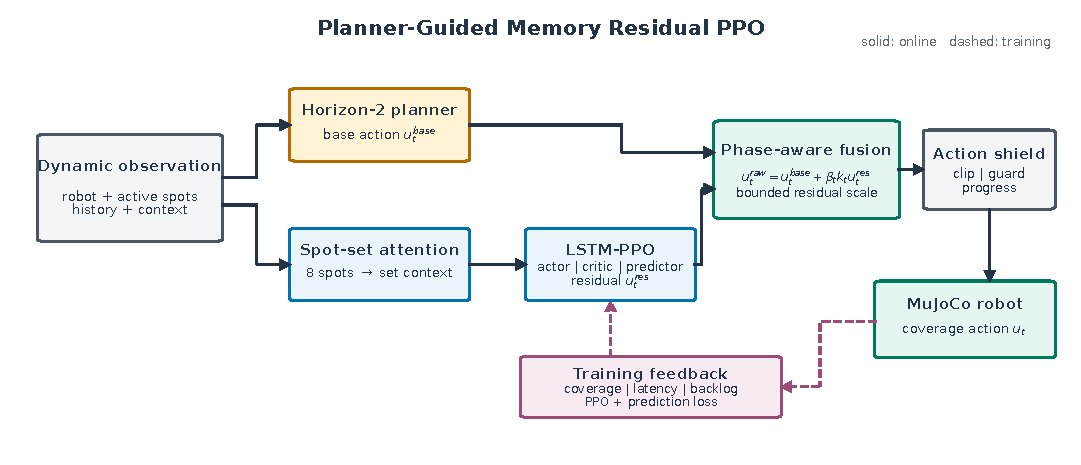
\includegraphics[width=0.86\textwidth]{figures/method_framework.pdf}
\caption{Planner-guided residual control. The online planner remains in the
action loop; LSTM-PPO supplies a bounded correction and the shield checks local
progress before the action is sent to the MuJoCo robot.}
\label{fig:framework}
\end{figure*}

\section{Introduction}
This work is motivated by robot-assisted loading and steaming of a granular
bed. Localized steam breakthroughs are detected by an external thermal sensing
system, and an ABB manipulator moves a deposition or coverage center over the
vessel to serve each active location. The simulator supplies target
coordinates, so the paper evaluates online control and service routing rather
than camera perception. Targets arrive in spatially clustered burst--lull
cycles, remain active until covered, and can accumulate while the arm is in
transit. This makes the task a persistent service problem: geometric travel,
waiting time, target age, and congestion must be considered together.

The problem is related to coverage path planning~\cite{galceran2013survey},
coverage control~\cite{cortes2004coverage}, statistical coverage
~\cite{arslan2019statistical}, and persistent monitoring with stochastic
arrivals~\cite{yu2015persistent}. It also has a direct connection to
stochastic dynamic vehicle routing, where online arrivals and waiting time
determine service quality~\cite{bertsimas1991stochastic,bertsimas1993multiple}.
Unlike static map coverage, an active spot leaves the queue only after physical
coverage. Reinforcement learning has been applied to adaptive coverage
planning~\cite{carvalho2025zeroshot,champagnie2024online}, but a visible-target
planner is already a competitive deterministic prior in this task. Residual reinforcement
learning~\cite{johannink2019residual} and bounded residual control
~\cite{yan2025ictrl,zhang2023robodact} provide a conservative way to retain
that prior. The set encoder follows the permutation-invariant motivation of
Set Transformer~\cite{lee2019settransformer}.

The paper is aligned with ICCC Track 6 (Robotics), with secondary links to
Tracks 2 (AI for Engineering) and 4 (Machine Learning). We ask:
\emph{RQ1}: does a bounded residual action interface improve a fixed planner
relative to a matched absolute-action PPO controller? \emph{RQ2}: how does
the method compare with alternative planner and heuristic priors? \emph{RQ3}:
what coverage--service trade-off is created in latency, strict SLA, backlog,
and smoothness?

Learning does not replace planning; it learns a correction around an online
route prior. The contributions are (i) a persistent thermal-spot service
formulation with explicit metric denominators, (ii) an LSTM-PPO residual
interface with phase-scaled authority and a progress shield, and (iii) a
crossed held-out evaluation that separates the residual interface from
auxiliary modules.

\section{Task and Method}
\subsection{Persistent service and metrics}
Let $\mathcal S_t=\{p_i(t)\}$ be the active spot set, where
$p_i=(x_i,y_i,a_i)$ contains location and active age, and let
$c_t=(x_t,y_t)$ be the coverage center. Spot $i$ is served when
\begin{equation}
\|c_t-(x_i,y_i)\|_2\le r_{\mathrm{cover}}.
\end{equation}
The spot is then removed. Timeout removal is disabled in the reported
protocol; an uncleared spot remains in the denominator. The action
$u_t=[\Delta x_t,\Delta y_t,s_t]\in[-1,1]^3$ is issued every $0.05$ s; the
MuJoCo integrator uses a $0.002$ s physics step.
Coverage is
\begin{equation}
C=\frac{N_{\mathrm{covered}}}{N_{\mathrm{spawned}}}.
\end{equation}
For a covered spot, $T_i=(n_i^{\mathrm{cover}}-n_i^{\mathrm{spawn}})
\times0.05$ s and $\bar T=N_{\mathrm{covered}}^{-1}\sum_iT_i$. Mean latency
and p90 are conditional on covered spots; p90 is the empirical 90th
percentile of the episode-level covered-spot latency list. Strict SLA exposes
the uncleared tail:
\begin{equation}
C_{\mathrm{SLA}}=\frac{|\{i:T_i\leq T_{\mathrm{SLA}}\}|}{N_{\mathrm{spawned}}},
\qquad T_{\mathrm{SLA}}=4.0\ \mathrm{s}.
\end{equation}
Backlog is the time-average active count; smoothness is
$\Delta_u=T^{-1}\sum_t\|u_t-u_{t-1}\|_2$. Metrics are aggregated within
evaluation cells before hierarchical resampling, with coverage primary.

\subsection{Planner prior and recurrent residual}
The interpretable risk score used by the comparator and as a diagnostic is
\begin{equation}
q_i=0.40\phi_{\mathrm{age}}+0.30\phi_{\mathrm{dist}}
    +0.10\phi_{\mathrm{reach}}+0.20\phi_{\mathrm{therm}}.
\end{equation}
For center $c_t$, potential radius $R_{\mathrm{pot}}$, home position
$p_{\mathrm{home}}$, maximum target offset $R_{\max}$, and stage age scale
$A_{\mathrm{norm}}$, the components are
\begin{align}
\phi_{\mathrm{age}}&=\operatorname{clip}(a_i/A_{\mathrm{norm}},0,1),\nonumber\\
\phi_{\mathrm{dist}}&=1-\operatorname{clip}(\|p_i-c_t\|/R_{\mathrm{pot}},0,1),\nonumber\\
\phi_{\mathrm{reach}}&=1-\operatorname{clip}(\|p_i-p_{\mathrm{home}}\|/R_{\max},0,1),\nonumber\\
\phi_{\mathrm{therm}}&=\operatorname{clip}(H(p_i),0,1).
\end{align}
The implementation also exposes
$\phi_{\mathrm{mat}}=\operatorname{clip}(\operatorname{mean}_g
[\max(H^*-H_g,0)\exp(-\|x_g-p_i\|^2/(2\sigma_d^2))]/H^*,0,1)$.
Here $x_g$ is the center of grid cell $g$, $H_g$ is its height, $H^*$ is the
target layer height, and $\sigma_d=0.18$ m is the deposition-kernel width;
the mean is taken over the grid.
The thermal score is
$H(p)=\operatorname{clip}(\sum_\ell a_\ell\exp(-\|p-h_\ell\|^2/(2\sigma_h^2)),0,1)$,
where $h_\ell$ and $a_\ell$ are hotspot centers and amplitudes and
$\sigma_h=0.22$ m. V12 disables urgency augmentation, so it does not enter
either $q_i$ or the H2 objective.
When material observation is enabled, the weights are
$(.35,.25,.15,.10,.15)$ for age, distance, material, reachability, and
thermal context; when it is disabled, they are
$(.40,.30,0,.10,.20)$.
The reported V12 protocol sets
\texttt{material\_observation=false}, hence
$\phi_{\mathrm{mat}}=0$ and its weight is zero. The risk-aware baseline is
stateless: it selects the first active-set entry attaining the maximum score
and outputs the normalized direction toward that target with speed one.

Horizon-$L$ enumerates ordered routes of length $\min(L,N_t)$. For route
$\rho=(i_1,\ldots,i_L)$, the planner simulates travel in steps and uses
\begin{align}
g_j &= q_{i_j}+0.45z_j-0.018d_j-0.050(z_j-1)_+,\nonumber\\
J(\rho) &= \sum_{j=1}^{L}0.82^{j-1}g_j-0.08\bar z_{\mathrm{left}},
\end{align}
where $d_j$ is travel steps and $z_j$ is arrival age normalized by
$A_{\mathrm{norm}}$; the simulated center and elapsed travel time are updated
after each route element. H2 uses $L=2$ and executes the first action of the
highest-scoring route; H3 uses the identical objective with $L=3$. The
planner enumerates all ordered routes from the active set, uses
$d_j=\max(1,\lceil\max(\|p_{i_j}-c\|-r_{\mathrm{cover}},0)/0.04\rceil)$,
and retains the first enumerated route under an exact tie. The resulting
action is the normalized direction to the first route target with speed one,
clipped to $[-1,1]^3$. Before execution, the environment applies action
smoothing $\bar u_t=0.7\bar u_{t-1}+0.3\tilde u_t$. For raw action
$u_t^{\mathrm{raw}}=[d_x,d_y,d_s]$, the planar displacement is
$0.04\,\eta_t[d_x,d_y]$, where
$\eta_t=0.65+0.35(d_s+1)/2$. Nearest, oldest, distance--age,
dynamic-weighted, ACO-TSP, and planner-ensemble baselines use the same
workspace, action interface, persistence rule, and coverage condition.

\begin{table}[t]
\caption{Horizon-2 target-selection procedure}
\label{tab:h2algorithm}
\centering\scriptsize
\begin{tabular}{@{}p{0.96\columnwidth}@{}}
\toprule
\textbf{Input:} active set $\mathcal S_t$, center $c_t$, and $L=2$.\\
1. Enumerate $\mathcal R_t=\operatorname{Perm}(\mathcal S_t,\min(2,|\mathcal S_t|))$ and evaluate $J(\rho)$ for each route.\\
2. Set $\rho^*=\arg\max J(\rho)$; strict $>$ preserves enumeration order on ties.\\
3. Output the normalized direction to $p_{\rho^*_1}$ with speed one, clipped to $[-1,1]^3$.\\
4. Recompute at the next decision step; no planner hidden state is carried.\\
\bottomrule
\end{tabular}
\end{table}

The observation has $61+8\times8=125$ features. The global branch is
$61\rightarrow256$ with LayerNorm and ReLU. Eight spot slots are embedded
with a shared $8\rightarrow128$ map and four-head masked attention; the pooled
spot branch is $128\rightarrow256$ with LayerNorm and ReLU. Their concatenation
is fused by $512\rightarrow256\rightarrow256$ LayerNorm--ReLU blocks and fed
to a one-layer width-256 LSTM. The fused representation
is processed by $256\rightarrow3$ actor, $256\rightarrow1$ critic, and
$256\rightarrow128\rightarrow2$ prediction heads. Actor means use tanh and
the state-independent log standard deviation is initialized to $-0.8$.
Relative target and active-spot coordinates and distances are divided by the
pot radius; ages are divided by $A_{\mathrm{norm}}$; thermal, material, risk,
coverage, route, and spawn-readiness features use bounded physical scales.
Joint coordinates and end-effector tracking errors remain in simulator units,
and actions are bounded in $[-1,1]$. No running test-set observation
normalizer is used. The hidden state is carried across rollout chunks and
coverage events, reset after a miss and at an episode boundary.
With planner action $u_t^{\mathrm{base}}$ and residual
$u_t^{\mathrm{res}}=\pi_\theta(o_t,h_t)$, the candidate is
\begin{align}
\tilde u_t &= \operatorname{clip}(u_t^{\mathrm{base}}+
\beta_t k_tu_t^{\mathrm{res}},-1,1),\nonumber\\
\beta_t &= 0.03+0.17\operatorname{clip}(n_t/700000,0,1).
\end{align}
The phase multipliers $(k_t)$ for lull, sparse, charging, mid, dense, and
burst are $(1.35,1.25,1.00,1.00,0.40,0.25)$. The post-policy shield rejects
alignment below $0.15$, requires candidate progress of at least $0.35$ of
base progress with margin $0.002$, and uses a 0.70-base/0.30-candidate
guarded blend with a $0.50$ progress ratio. Reverse turns below cosine
$-0.55$ are blended, and a candidate worse than the base is rejected after
90 no-cover steps. It is a local progress filter, not a formal temporal-logic
safety guarantee~\cite{alshiekh2018shielding}.

The scalarized reward contains time, active count, mean age, potential,
best progress, coverage, quick cover, precision, latency, oldest active,
backlog, SLA, action change, action norm, miss, and success terms. The
stage base cover, quick-cover, and potential values are
$(68,64,62,60)$, $(16,14,12,10)$, and $(8.0,7.5,6.5,5.8)$; the V12 scale
factors are $(.70,3.0,.65,.65,.45,2.4,2.8)$ for cover, quick cover,
precision, potential, best progress, active count, and age. Thus the
corresponding scaled coefficients are cover $(47.6,44.8,43.4,42.0)$,
quick cover $(48,42,36,30)$, precision $7.8$, potential
$(5.20,4.875,4.225,3.77)$, best progress $.3375$, active count $.024$,
and age $.112$. The remaining coefficients are
$r_{\mathrm{time}}=(.030,.035,.045,.055)$,
$r_{\mathrm{latency}}=30$, $r_{\mathrm{oldest}}=.45$,
$r_{\mathrm{backlog}}=.20$, $r_{\mathrm{SLA}}=(20,-30)$,
$r_{\Delta u}=.025$, $r_{\|u\|}=.004$, $r_{\mathrm{miss}}=28$, and
$r_{\mathrm{success}}=30$. The timeout-miss term is inactive because timeout
removal is disabled. The reward is multiplied by $0.02$ and clipped to
$[-4,4]$; SLA and backlog are therefore scalar preferences, not hard
constraints. The success bonus is emitted when covered count reaches the
stage target and coverage reaches the configured target coverage.

\begin{figure}[t]
\centering
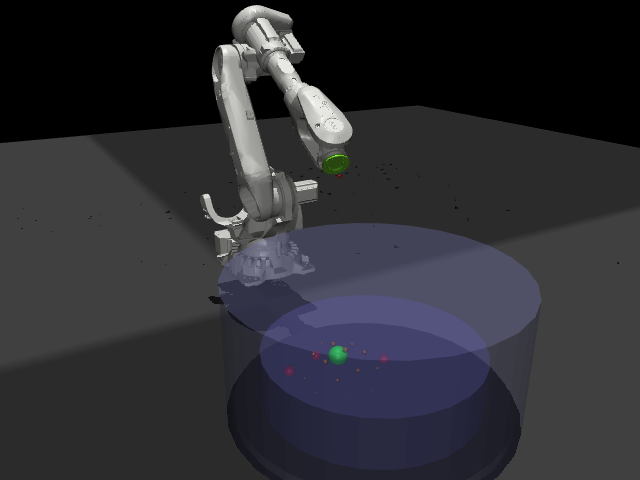
\includegraphics[width=0.37\columnwidth]{figures/mujoco_environment_snapshot.png}\hfill
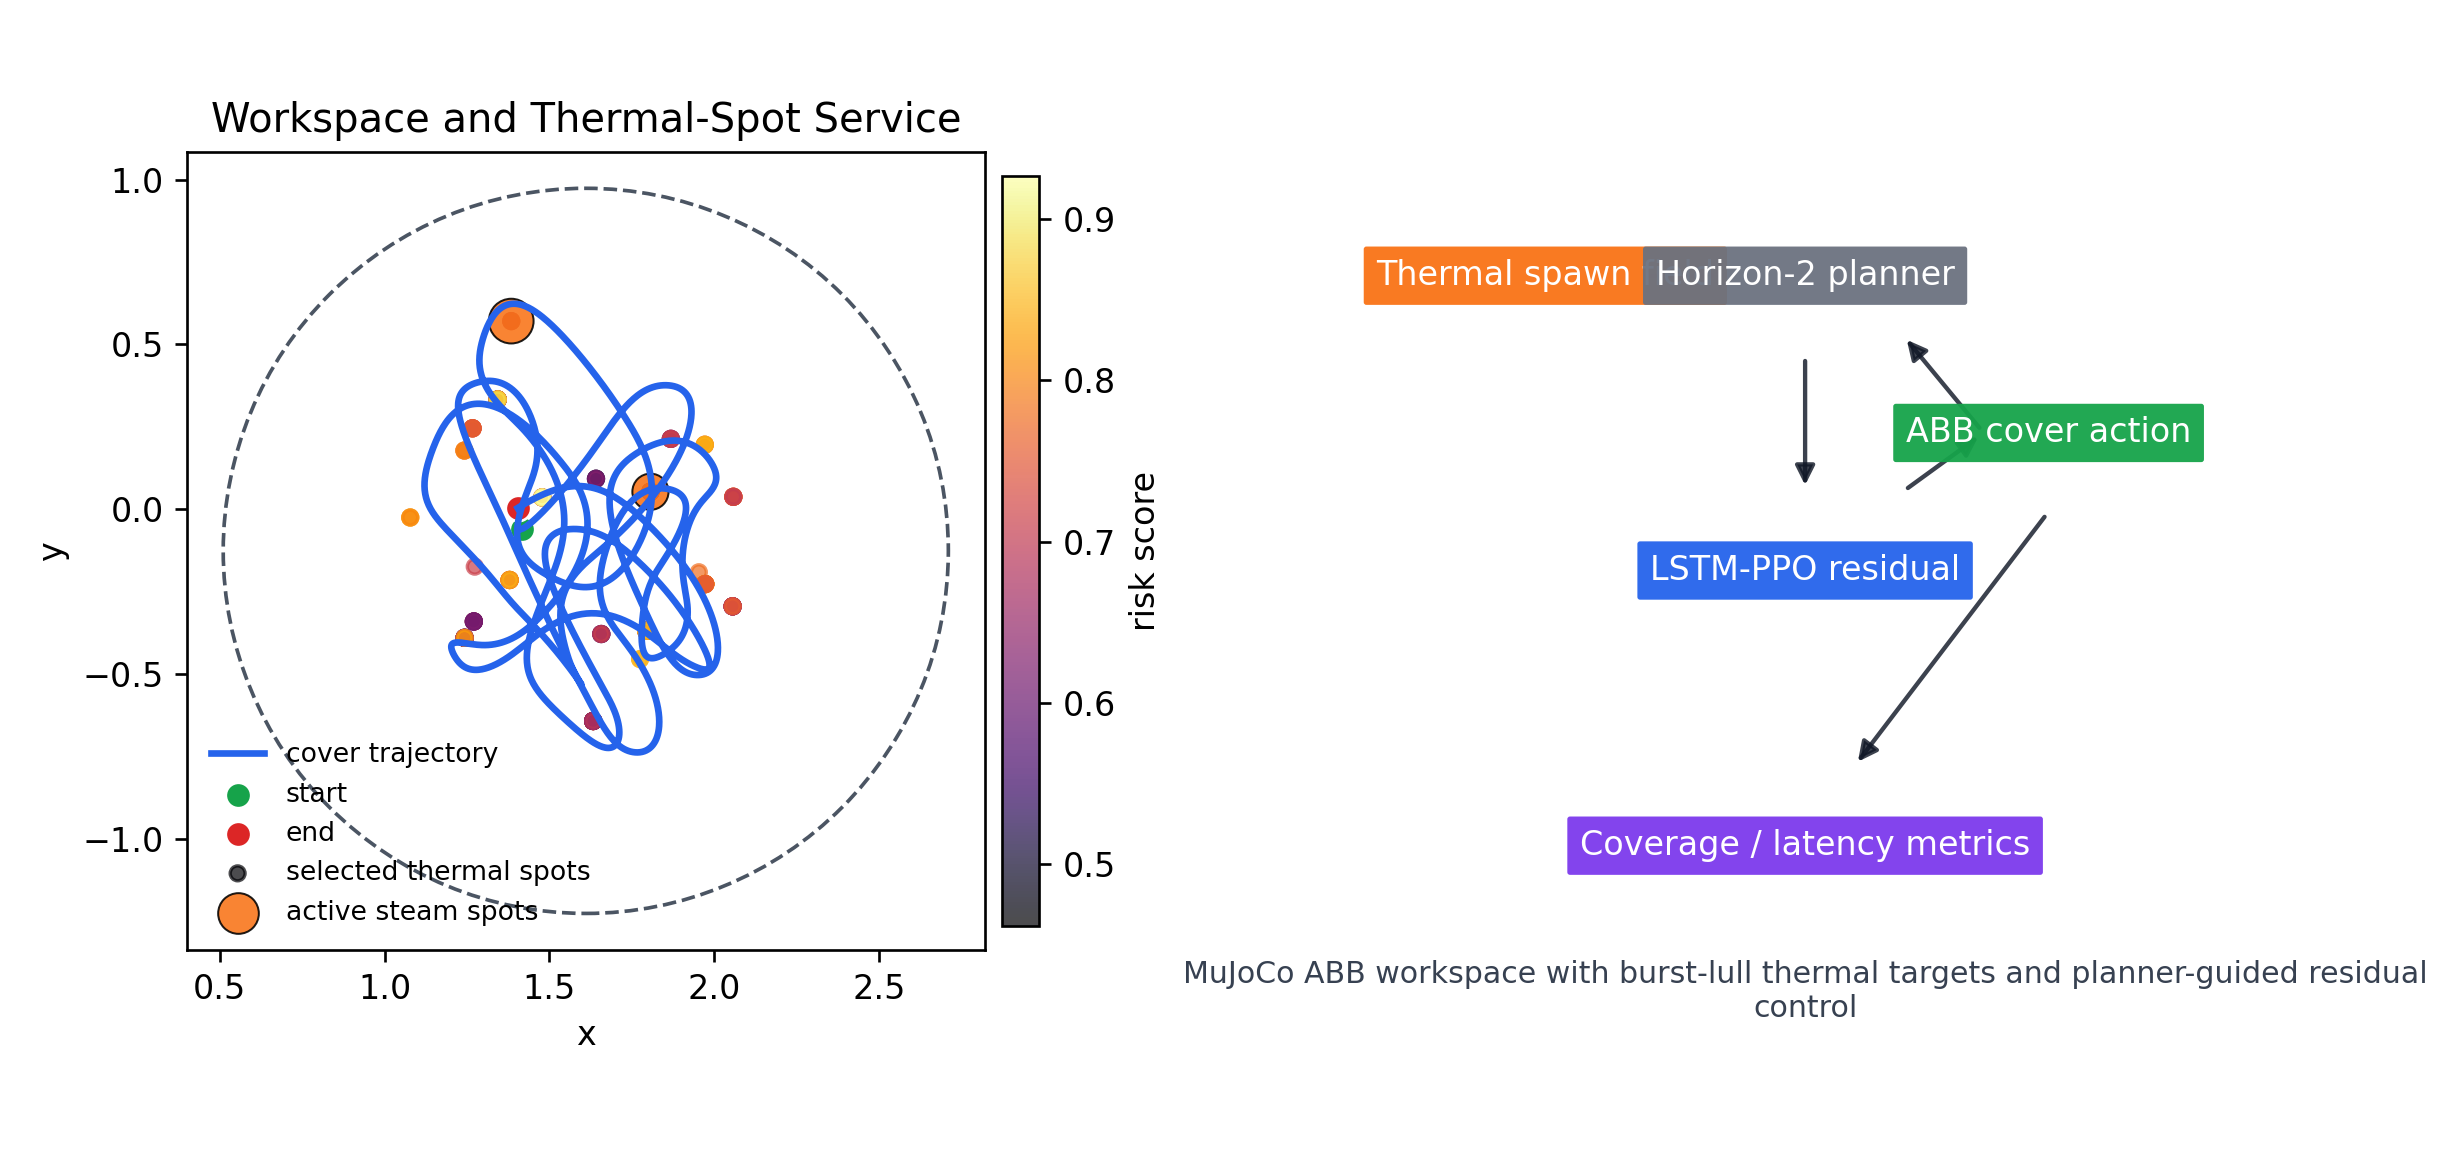
\includegraphics[width=0.60\columnwidth]{figures/mujoco_task_overview.png}
\caption{MuJoCo ABB workspace (left) and online thermal-spot service task
(right). The controller moves the green coverage center over clustered spots
inside the circular vessel.}
\label{fig:task}
\end{figure}

\section{Experiments}
\subsection{Protocol and statistical unit}
The MuJoCo twin~\cite{mujoco2012physics} contains an ABB arm, circular vessel,
and external target field. Three drifting hotspots generate a 70-step lull,
110-step charge, then 3--5 spots emitted every four steps; background and
strength are 0.055 and 3.8. Each learned method uses train seeds $0$--$2$,
held-out seeds $100$--$102$, five 3,200-decision-step episodes per crossed
cell, and the terminal checkpoint after a fixed curriculum. The training
budget is $1,152\times800=921,600$ decision steps per seed. PPO uses
$(\gamma,\lambda)=(.985,.95)$, Adam with $10^{-5}$ learning rate and
$\epsilon=10^{-5}$, one epoch, clips $(.05,.05)$, value coefficient $.5$,
gradient norm $.35$, entropy
$8\times10^{-4}\rightarrow1.8\times10^{-4}$ over $10^6$ steps, curriculum
80/160/720/192 episodes from Low to Extreme, H2 BC for 200 episodes
(20/40/100/40), 12 BC epochs, prediction coefficient $.05$ with a 150-step horizon, BC
decay $0.03\rightarrow0$ over 260,000 steps, and residual schedule
$0.03\rightarrow0.20$ over 700,000 steps. The PPO objective additionally
uses action-smooth and action-$\ell_2$ coefficients $(.02,.002)$; advantages
are standardized within each update. The budget therefore contains
$921,600/3,200=288$ PPO updates. Checkpoints are written every 50
training episodes and at curriculum-stage boundaries; the reported file is
the terminal
\texttt{scheme\_d\_paper\_base\_latest\_full.pt} written after episode 1,152.
Held-out data do not select checkpoints. Matched component variants use the
same fixed V12 settings, budget, and action interface; no common hyperparameter
search was completed. The historical Vanilla diagnostic was not independently
retuned under a full-budget protocol. The archived
`episodes.csv` files record reward, coverage, SLA, residual scale, recurrent
counters, prediction events, and elapsed steps.

The reported evaluation uses a fixed 3,200-decision-step service window,
equivalent to 160 s at $0.05$ s per decision. Timeout removal and
terminal drain-to-clear are disabled in this protocol; an active but
uncovered spot remains in the denominator and contributes to the pending
backlog at the window boundary.

Each episode first yields coverage, latency, SLA, backlog, and smoothness
values; p90 is computed from that episode's covered-spot latency list and is
not recomputed by pooling spots across episodes. Cell summaries average the
five episodes, and the balanced crossed design is then summarized over
training and held-out environment seeds. We use 20,000 crossed bootstrap
draws: training labels, evaluation labels, and episodes are resampled at their
respective levels, while paired methods reuse the same held-out scenarios.
Deterministic planners omit the training-seed level. Tables report
hierarchical 95\% intervals; Holm correction is applied across the four
stages for each predeclared comparison family. This keeps training randomness
and environment randomness from being treated as 45 independent flat
observations.

\begin{table}[t]
\caption{Stage and training parameters}
\label{tab:stage}
\centering\scriptsize\setlength{\tabcolsep}{2.5pt}
\begin{tabular}{@{}lrrrrr@{}}
\toprule
Stage & $N_{\max}$ & $r_{\rm cover}$ & $A_{\rm norm}$ & $p_{\rm spawn}$ & cooldown\\
\midrule
Low & 3 & .17 & 260 & .006 & 80\\
Realistic & 4 & .14 & 220 & .010 & 65\\
Hard & 6 & .12 & 200 & .018 & 48\\
Extreme & 8 & .10 & 180 & .026 & 36\\
\midrule
Obs. / widths & \multicolumn{5}{l}{$125$; spot 128, global/LSTM 256; 4-head attention}\\
Sequence / update & \multicolumn{5}{l}{$4\times800=3200$; PPO update every 4 chunks}\\
\bottomrule
\end{tabular}
\end{table}

\subsection{Coverage and baselines}
Table~\ref{tab:main} is the primary comparison. Ours is not distinguishable
from H2 in the first three stages; the Extreme interval is positive before,
but not after, four-stage Holm correction. Risk-aware has a higher point
estimate in Extreme, while H3 and the planner ensemble have comparable point
estimates in selected stages. Its
non-monotonic coverage $(.924,.901,.836,.863)$ follows from jointly changing
capacity, radius, arrival rate, and $A_{\mathrm{norm}}$; it has no hidden state.

\begin{table}[t]
\caption{Coverage versus Horizon-2 (hierarchical 95\% CIs)}
\label{tab:main}
\centering\scriptsize\setlength{\tabcolsep}{1.5pt}
\resizebox{\columnwidth}{!}{%
\begin{tabular}{@{}lccccc@{}}
\toprule
Stage & Ours & H2 & $\Delta$ & $\Delta$ CI & $p_{\rm Holm}$\\
\midrule
Low & .917 [.906,.929] & .919 [.906,.932] & -.002 & [-.018,.016] & 1.000\\
Real. & .901 [.884,.922] & .896 [.883,.910] & +.005 & [-.018,.034] & 1.000\\
Hard & .870 [.844,.894] & .870 [.847,.894] & $<.001$ & [-.040,.033] & 1.000\\
Extreme & .855 [.828,.881] & .816 [.782,.849] & +.038 & [.003,.074] & .135\\
\bottomrule
\end{tabular}}
\end{table}

\begin{figure}[t]
\centering
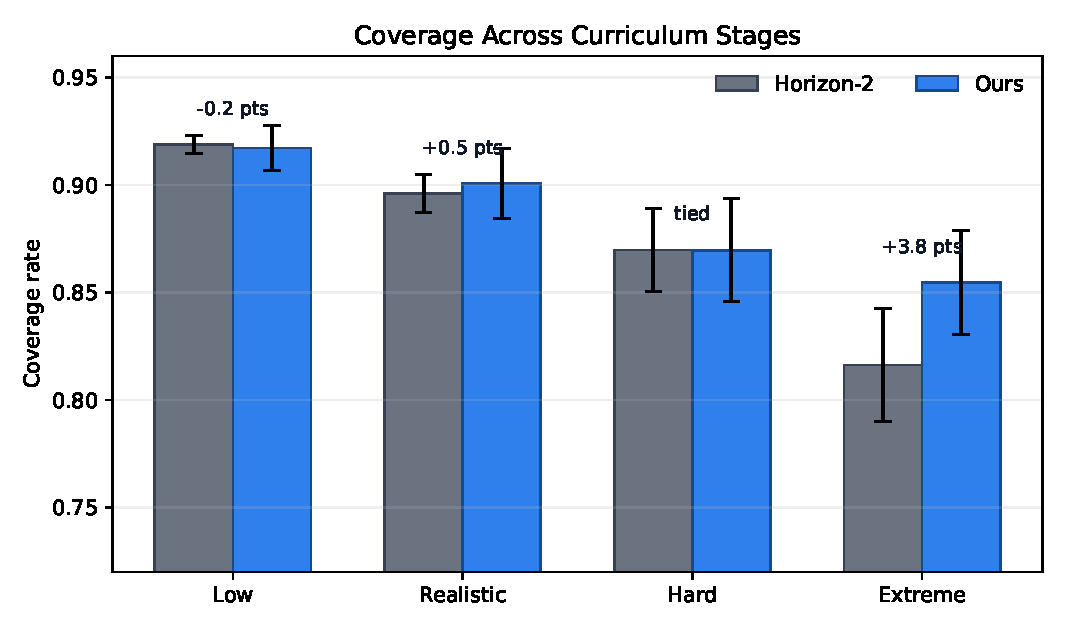
\includegraphics[width=\columnwidth]{figures/main_coverage_ours_vs_horizon2.pdf}
\caption{Stage-wise coverage with hierarchical 95\% intervals. The separation
is concentrated in Extreme and does not remain significant after correction.}
\label{fig:coverage}
\end{figure}

\begin{table}[t]
\caption{Coverage across deterministic and learned baselines. Brackets are
hierarchical 95\% CIs; $\pm$ values are evaluation-seed standard deviations.}
\label{tab:baselines}
\centering\tiny\setlength{\tabcolsep}{1.2pt}
\resizebox{\columnwidth}{!}{%
\begin{tabular}{@{}lcccc@{}}
\toprule
Method & Low & Real. & Hard & Extreme\\
\midrule
Ours & .917 [.906,.929] & .901 [.884,.922] & .870 [.844,.894] & .855 [.828,.881]\\
Horizon-2 & .919 [.906,.932] & .896 [.883,.910] & .870 [.847,.894] & .816 [.782,.849]\\
Horizon-3 & .917$\pm$.009 & .927$\pm$.025 & .860$\pm$.022 & .841$\pm$.060\\
Risk-aware & .924 [.902,.953] & .901 [.885,.918] & .836 [.778,.876] & .863 [.833,.892]\\
Nearest & .922$\pm$.011 & .887$\pm$.016 & .860$\pm$.026 & .789$\pm$.050\\
Oldest & .914$\pm$.004 & .890$\pm$.014 & .883$\pm$.019 & .807$\pm$.032\\
Distance--age & .921$\pm$.016 & .896$\pm$.008 & .851$\pm$.020 & .801$\pm$.065\\
Dynamic weighted & .927$\pm$.003 & .886$\pm$.023 & .865$\pm$.005 & .799$\pm$.045\\
ACO-TSP & .925$\pm$.006 & .893$\pm$.004 & .864$\pm$.033 & .754$\pm$.061\\
Planner ensemble & .935$\pm$.012 & .899$\pm$.014 & .870$\pm$.003 & .814$\pm$.090\\
No residual & .838 [.712,.915] & .776 [.667,.865] & .726 [.590,.837] & .687 [.585,.793]\\
Vanilla LSTM-PPO & .166 [.067,.286] & .130 [.048,.234] & .089 [.025,.181] & .061 [.017,.115]\\
\bottomrule
\end{tabular}}
\\[-2pt]
\raggedright\footnotesize The deterministic rows use the same environment
seeds and action interface; Horizon-$L$ uses the objective defined above.
Vanilla is reported as a descriptive diagnostic because its training protocol
is confounded, not as a causal baseline.
\end{table}

\subsection{Action-interface and component evidence}
The matched No-residual policy retains the observation, LSTM, H2 warm start,
prediction loss, service reward, and budget, but emits an absolute action
without a planner base or shield. This is the controlled action-interface
comparison. Historical Vanilla LSTM-PPO changes residual composition, BC, and
prediction jointly, and was not independently retuned under a full-budget
protocol; it is descriptive rather than causal. Table~\ref{tab:diagnostic_panels}(b)
records the differences.

\subsection{Service diagnostics and robustness}
Table~\ref{tab:diagnostic_panels}(c) reports service cost. In Extreme, the
$0.038$ coverage increase has $2.50$ s higher mean latency, $6.09$ s higher
p90, $0.26$ more active spots, and lower strict SLA. On an unseen
higher-density condition, ours obtains .868/.850 in Hard/Extreme and H2
.888/.825; overlapping intervals make this robustness evidence. H3 tests
planner capacity only; matched H3-residual retraining is not claimed.

\begin{table*}[t]
\caption{Mechanism and service evidence: (a) matched residual-interface
effect, (b) component accounting, and (c) coverage--service diagnostics.}
\label{tab:diagnostic_panels}
\centering\scriptsize
\begin{minipage}[t]{0.485\textwidth}
\centering
\textbf{(a) Matched residual-interface effect}\\[2pt]
\setlength{\tabcolsep}{1.8pt}
\resizebox{\linewidth}{!}{%
\begin{tabular}{@{}lccccc@{}}
\toprule
Stage & Full & No residual & $\Delta$ & $\Delta$ CI & $p_{\rm Holm}$\\
\midrule
Low & .917 & .838 [.712,.915] & +.079 & [.004,.202] & .029\\
Real. & .901 & .776 [.667,.865] & +.124 & [.036,.223] & .003\\
Hard & .870 & .726 [.590,.837] & +.144 & [.037,.268] & .011\\
Extreme & .855 & .687 [.585,.793] & +.168 & [.050,.285] & .003\\
\bottomrule
\end{tabular}}\\[3pt]
\textbf{(b) Exact component accounting}\\[2pt]
\setlength{\tabcolsep}{1.7pt}
\resizebox{\linewidth}{!}{%
\begin{tabular}{@{}lccccccc@{}}
\toprule
Variant & Action & BC & Attn. & Carry & Pred. & Svc. & Shield\\
\midrule
Full & H2+res. & Y & Y & Y & Y & Y & Y\\
No residual & absolute & Y & Y & Y & Y & Y & N\\
No attention & H2+res. & Y & N & Y & Y & Y & Y\\
No carry & H2+res. & Y & Y & N & Y & Y & Y\\
No prediction & H2+res. & Y & Y & Y & N & Y & Y\\
No service & H2+res. & Y & Y & Y & Y & N & Y\\
Vanilla & absolute & N & Y & Y & N & Y & N\\
\bottomrule
\end{tabular}}
\end{minipage}\hfill
\begin{minipage}[t]{0.485\textwidth}
\centering
\textbf{(c) Coverage and service diagnostics versus H2}\\[2pt]
\setlength{\tabcolsep}{2.2pt}
\resizebox{\linewidth}{!}{%
\begin{tabular}{@{}llrrrrrr@{}}
\toprule
Stage & Method & Cov. & Mean lat. (s) & p90 (s) & Strict SLA & Backlog & $\Delta_u$\\
\midrule
Low & Ours & .917 & 12.54 & 24.15 & .181 & 2.30 & .0254\\
 & H2 & .919 & 12.16 & 23.72 & .191 & 2.28 & .0255\\
Real. & Ours & .901 & 16.04 & 29.70 & .147 & 2.84 & .0261\\
 & H2 & .896 & 16.52 & 29.45 & .131 & 2.82 & .0258\\
Hard & Ours & .870 & 19.59 & 38.10 & .127 & 3.49 & .0277\\
 & H2 & .870 & 19.23 & 35.44 & .121 & 3.43 & .0274\\
Extreme & Ours & .855 & 23.88 & 46.01 & .103 & 3.81 & .0289\\
 & H2 & .816 & 21.38 & 39.92 & .128 & 3.55 & .0277\\
\bottomrule
\end{tabular}}
\vspace{1pt}

\raggedright\footnotesize Mean and p90 latency condition on covered spots;
strict SLA uses all spawned spots. Backlog is mean active count and $\Delta_u$
is mean per-step action change.
\end{minipage}
\end{table*}

\begin{figure*}[t]
\centering
\begin{tabular}{cc}
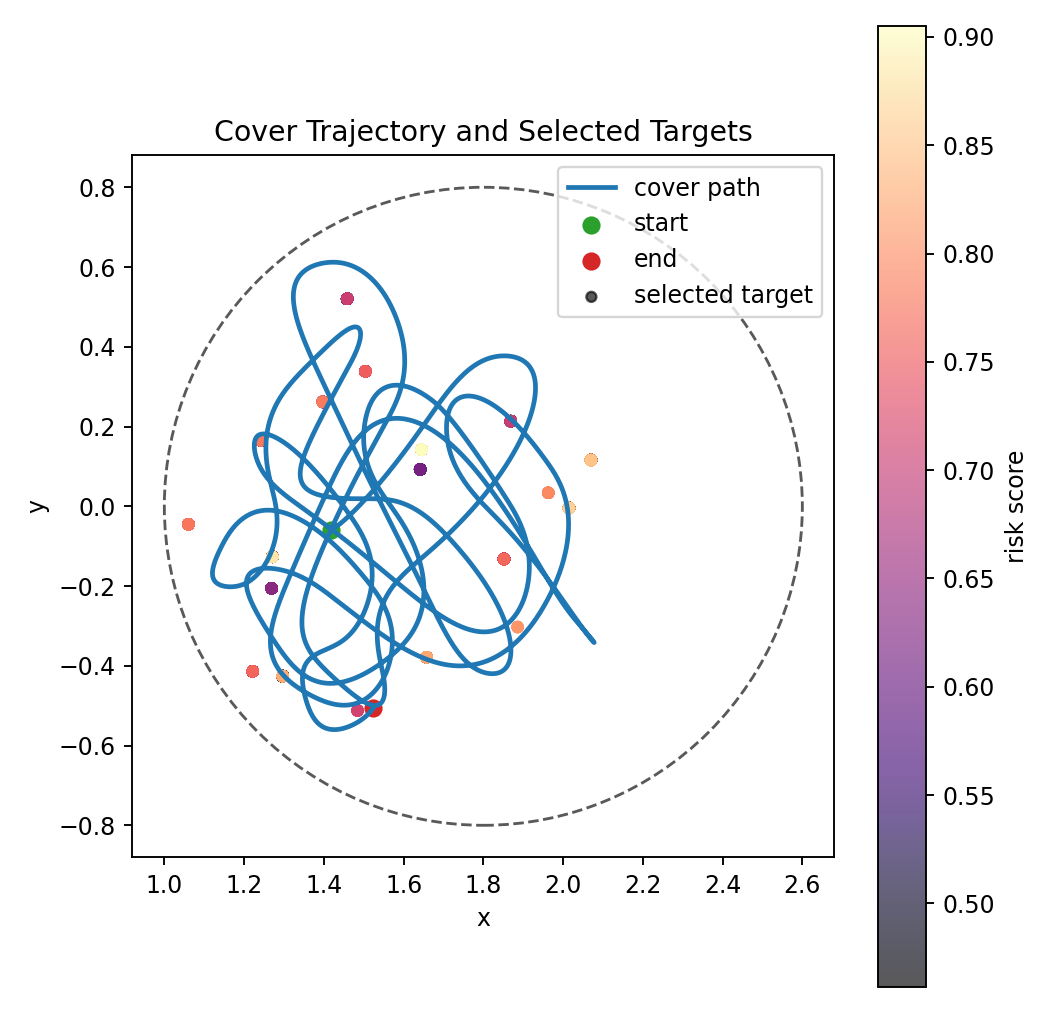
\includegraphics[width=0.25\textwidth]{figures/ours_realistic_trajectory.png} &
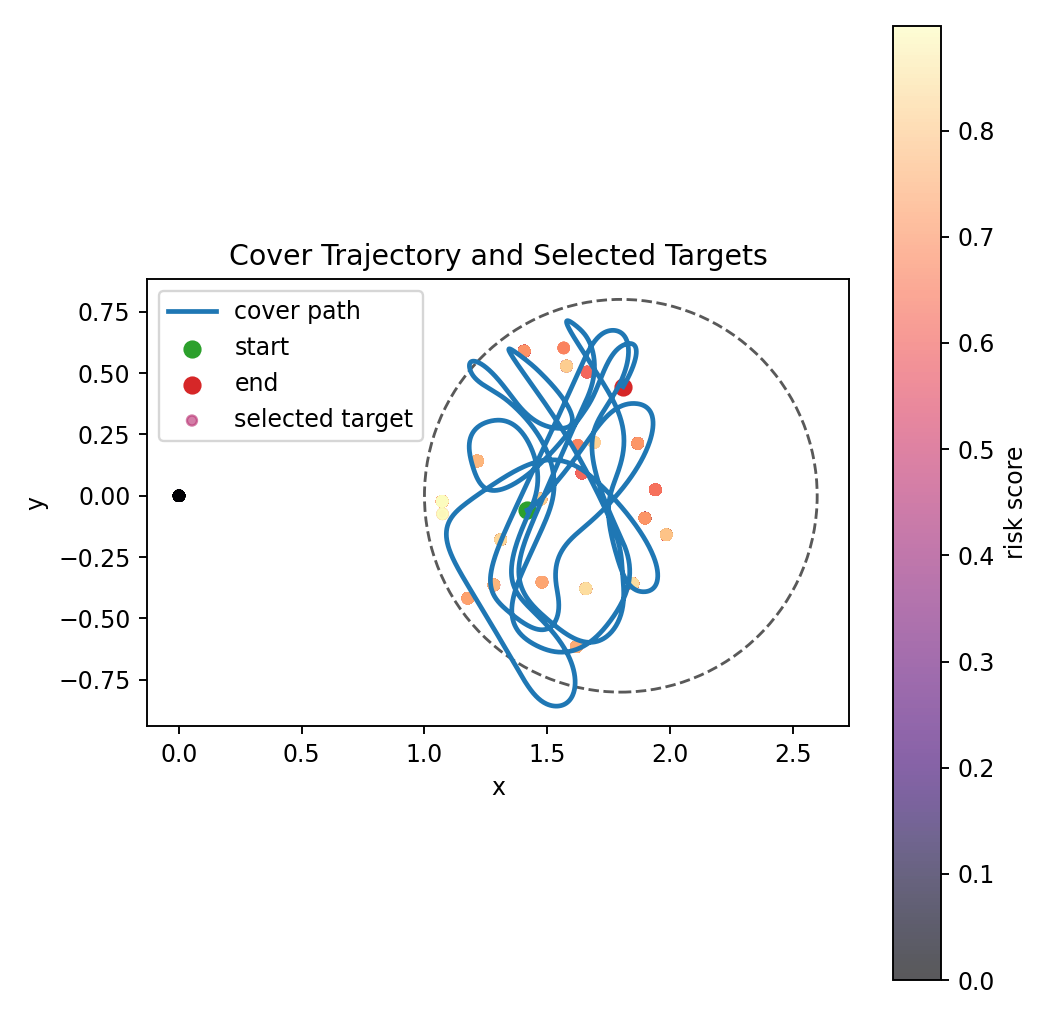
\includegraphics[width=0.25\textwidth]{figures/horizon2_realistic_trajectory.png}\\
(a) Planner-guided residual PPO & (b) Horizon-2
\end{tabular}
\caption{Representative held-out Realistic trajectories. Aggregate claims use
the crossed training/evaluation seed cells.}
\label{fig:trajectory}
\end{figure*}

\section{Discussion and Conclusion}
The matched action-interface comparison is consistent with a contribution from
the planner-residual interface; it does not establish dominance over H2 or
the risk-aware heuristic. H2 is not distinguishable from the learned method
in three stages, while the
Extreme difference is positive before but not after Holm correction. The
historical Vanilla result is confounded by simultaneous changes to residual
composition, BC, and prediction, and is therefore diagnostic only. The
auxiliary ablations do not establish independent gains for attention, carry,
prediction, or service shaping.

H3 evaluates deterministic planner capacity, not residual transfer, because
the learned controller was trained around H2. Finally, the $0.05$ s interval
measures task time rather than inference time, and the fixed window does not
enforce terminal clearance. The evidence therefore concerns fixed-horizon
persistent service; terminal-drain evaluation, matched H3-residual training,
and hardware timing remain future work.

\begingroup
\renewcommand{\footnotesize}{\tiny}
\makeatletter
\def\IEEEbibitemsep{-1pt}
\makeatother
\bibliographystyle{IEEEtran}
\bibliography{rl_robot_refs}
\endgroup

\end{document}
